\chapter{Compiladores}\label{chp:COMPILADORES}

Este capítulo apresenta a teoria fundamental relacionada à construção de compiladores. 
Serão esclarecidos os fundamentos da compilação, as etapas que compõem o processo,
os diferentes mecanismos de tipagem, e, por fim, um aprofundamento sobre a tipagem dinâmica.
Essas noções ajudarão na compreensão das decisões arquiteturais e soluções adotadas para o compilador Gary.


\section{O Processo de Compilação}

Linguagens de programação são notações que facilitam a escrita de software. 
Elas operam como uma camada de abstração com respeito à complexidade de lidar com o hardware,
além de facilitarem a compreensão humana por tornarem o código mais próximo à linguagem natural.
Entretanto, essa notação não é diretamente compreendida pela máquina.
Portanto, é necessário um software capaz de traduzir essa representação abstraída para um formato que o computador possa executar.
A esse software se dá o nome de compilador ou interpretador,
dependendo de como a tradução é feita \cite{aho2008compiladores}.

Pode-se definir um compilador como um software que recebe como entrada
um código escrito em uma linguagem de programação (a linguagem fonte) e
gera como saída uma representação, semanticamente idêntica, em outra linguagem (linguagem objeto).
Linguagem essa que pode já ser executável pela máquina ou, caso contrário,
ser uma linguagem de transição, denominada de \ac{RI} \cite{aho2008compiladores}.

A Figura~\ref{fig:repr_compiler} ilustra a representação abstraída de um compilador.

\begin{figure}[!htb]
    \centering
    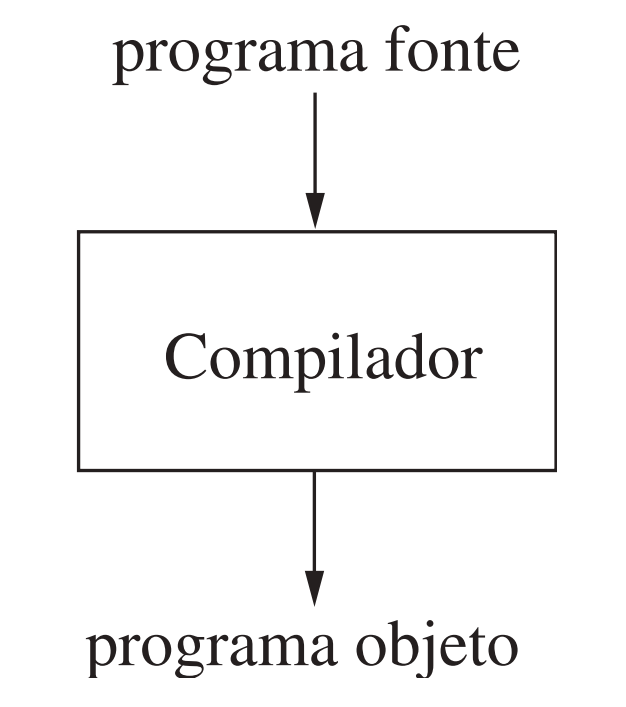
\includegraphics[width=0.3\textwidth]{imagens/Repr_Compiler.png}
    \caption{Representação simples de um compilador}
    \label{fig:repr_compiler}
    \legend{Fonte: Adaptado de \citeonline{aho2008compiladores}}
\end{figure}

Por sua vez, um interpretador é similar ao compilador, 
exceto pelo fato de que o interpretador não gera um programa objeto, em vez disso,
ele executa diretamente as instruções do programa fonte sobre as entradas do usuário \cite{aho2008compiladores}.

A Figura~\ref{fig:repr_interpreter} ilustra a representação abstraída de um interpretador.

\begin{figure}[!htb]
    \centering
    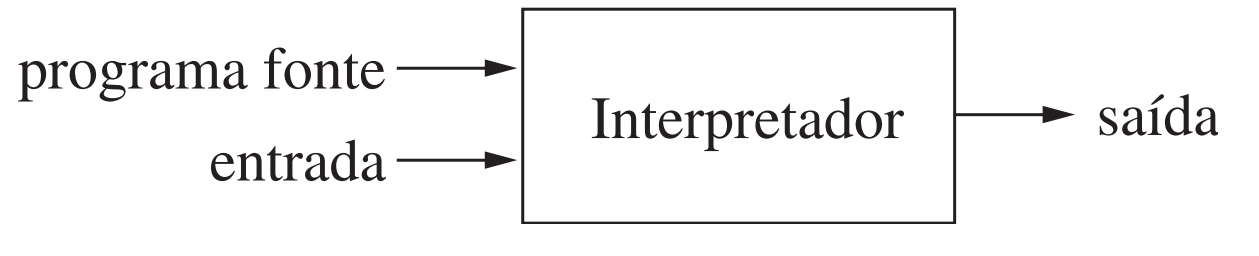
\includegraphics[width=0.6\textwidth]{imagens/Repr_Interpreter.png}
    \caption{Representação simples de um interpretador}
    \label{fig:repr_interpreter}
    \legend{Fonte: Adaptado de \citeonline{aho2008compiladores}}
\end{figure}

\citeonline{aho2008compiladores} destacam que a vantagem principal de um compilador 
sobre um interpretador é que, normalmente, após o programa ser traduzido pelo compilador,
ele executará muito mais rápido do que se estivesse sendo feito pelo interpretador. 
Por outro lado, a vantagem do interpretador é que, como ele executa instrução por instrução,
o diagnóstico do erro tende a ser superior.

Estabelecida a definição geral do processo de compilação, 
é necessário compreender como essa tradução estrutural ocorre na prática.
A conversão de um texto legível por humanos em instruções executáveis é uma tarefa de alta complexidade, 
razão pela qual o sistema é fragmentado em fases lógicas. 
A seção a seguir esclarece as principais etapas às quais o código-fonte é submetido
até a sua conversão em código-objeto.


\section{Fases de um Compilador}




\section{Sistema de Tipos}

\section{Tipagem Dinâmica na Compilação}